\documentclass[10pt,a4paper]{article}
\usepackage[T1]{fontenc}
\usepackage[utf8]{inputenc}
\usepackage[spanish,es-tabla]{babel}
\parindent=0cm %Modificar tamaño de sangria
\usepackage{amsmath}
\usepackage{amssymb,amsfonts,latexsym,cancel}
\usepackage{graphicx}
\usepackage{epstopdf}
\usepackage{float}
\usepackage{subfigure}
\usepackage{array}
\usepackage{longtable}
\newcolumntype{E}{>{$}c<{$}}
\setcounter{MaxMatrixCols}{40}
\usepackage{bm}
\usepackage{xcolor}
%%%%%%%%%%%%%%%%%%%%%%%%%%%%%%%%%%%%%
%%%PAQUETES O CONFIGURACION NUEVA%%%%
%%%%%%%%%%%%%%%%%%%%%%%%%%%%%%%%%%%%%
\usepackage[lmargin=2cm, rmargin=2cm,top=2.5cm,bottom=2cm]{geometry}
\usepackage{fancyhdr}
\pagestyle{fancy}
\fancyhead{}%%Es para limpiar el documento
\fancyhead[C]{Metaheurística}
\fancyhead[R]{
\includegraphics[scale=0.07]{figuras/logo}}
\fancyfoot{}
\fancyfoot[R]{\thepage}
\fancyfoot[L]{Bryan Ricardo}
\renewcommand{\headrulewidth}{0.9pt}
\renewcommand{\footrulewidth}{0.5pt}
\usepackage{xcolor}
\providecommand{\abs}[1]{\lvert#1\rvert}
\providecommand{\norm}[1]{\lVert#1\rVert}
\usepackage{ mathrsfs }
\usepackage{algorithm}
\usepackage{algpseudocode}
%%%%%%%%%%%%%%%%%%%%%%%%%%%%%%%%%%%%%
%%INTEGRALES INFERIORES Y SUPERIORES
\usepackage{amsmath}
\def\upint{\mathchoice%
    {\mkern13mu\overline{\vphantom{\intop}\mkern7mu}\mkern-20mu}%
    {\mkern7mu\overline{\vphantom{\intop}\mkern7mu}\mkern-14mu}%
    {\mkern7mu\overline{\vphantom{\intop}\mkern7mu}\mkern-14mu}%
    {\mkern7mu\overline{\vphantom{\intop}\mkern7mu}\mkern-14mu}%
  \int}
\def\lowint{\mkern3mu\underline{\vphantom{\intop}\mkern7mu}\mkern-10mu\int}
%%%%%%%%%%%%%%%%%%%%%%%%%%%%%%%%%%%%%%%%%%%%%%%
\begin{document}
\begin{titlepage}
\begin{center}
\vspace*{2\baselineskip}%%saltos de linea
\hrule height 3pt
\vspace*{0.5\baselineskip}%%saltos de linea
{\Huge \textbf{Universidad Autonoma de Aguascalientes}}
{\Large \textbf{LICENCIATURA EN MATEMATICAS APLICADAS}}
\vspace*{0.5\baselineskip}%%saltos de linea
\hrule
\vspace*{0.5\baselineskip}%%saltos de linea

\includegraphics[scale=0.5]{figuras/logo}
\vspace*{2\baselineskip} \\%%saltos de linea
\textbf{\large MATERIA: Metaheurística} \\
\vspace*{1.5\baselineskip}
\textbf{\large DOCENTE: EUNICE ESTHER PONCE DE LEON SENTI } \\
\vspace*{1.5\baselineskip}
\textbf{\large FECHA DE CREACION: 13 de agosto de 2023} \\  
\vspace*{3\baselineskip}
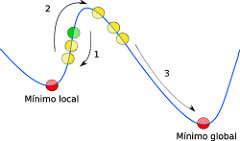
\includegraphics[scale=1.2]{figuras/imagen}
\vfill
BRYAN RICARDO BARBOSA OLVERA \\
\today \\

\end{center}
\end{titlepage}


\LARGE
\section{Pseudocodigo Criterio de la primera derivada}
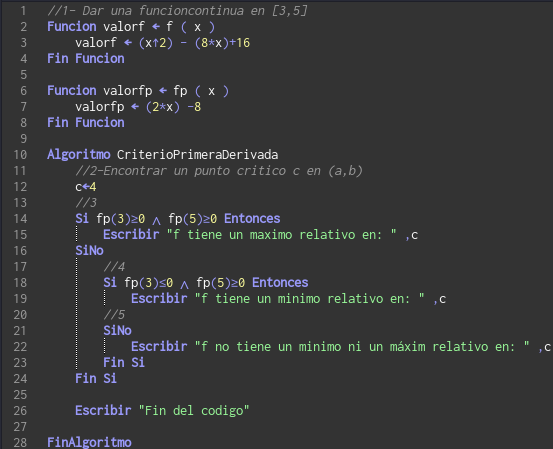
\includegraphics[scale=0.5]{figuras/img1} \\ 
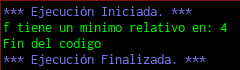
\includegraphics[scale=0.5]{figuras/img2}

\section{Criterio de la segunda derivada}

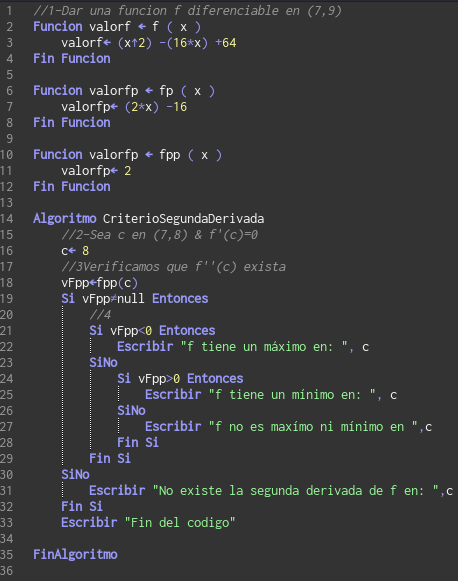
\includegraphics[scale=0.5]{figuras/img3} \\ 
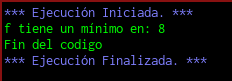
\includegraphics[scale=0.5]{figuras/img4}


\section{Criterio de maximos y minimos en funciones reales de variable vectorial}
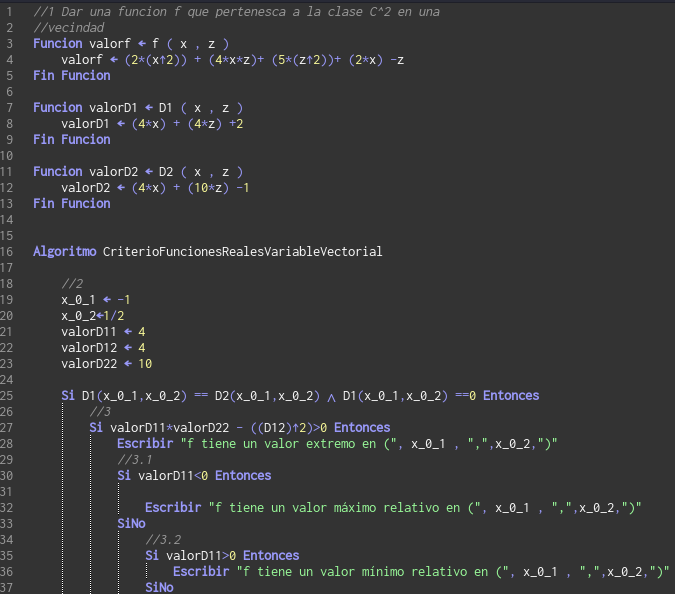
\includegraphics[scale=0.5]{figuras/img5}  \\ \\
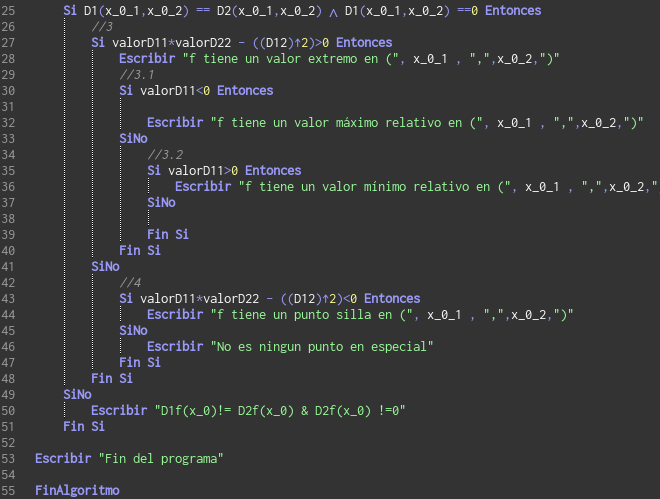
\includegraphics[scale=0.5]{figuras/img6}

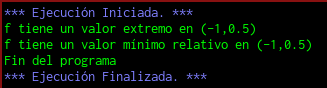
\includegraphics[scale=0.5]{figuras/img7}

\end{document}
